\section{Introduction}\label{sec:intro}

\begin{wrapfigure}[15]{r}{0.5\textwidth}
\vspace{-12pt}
\centering
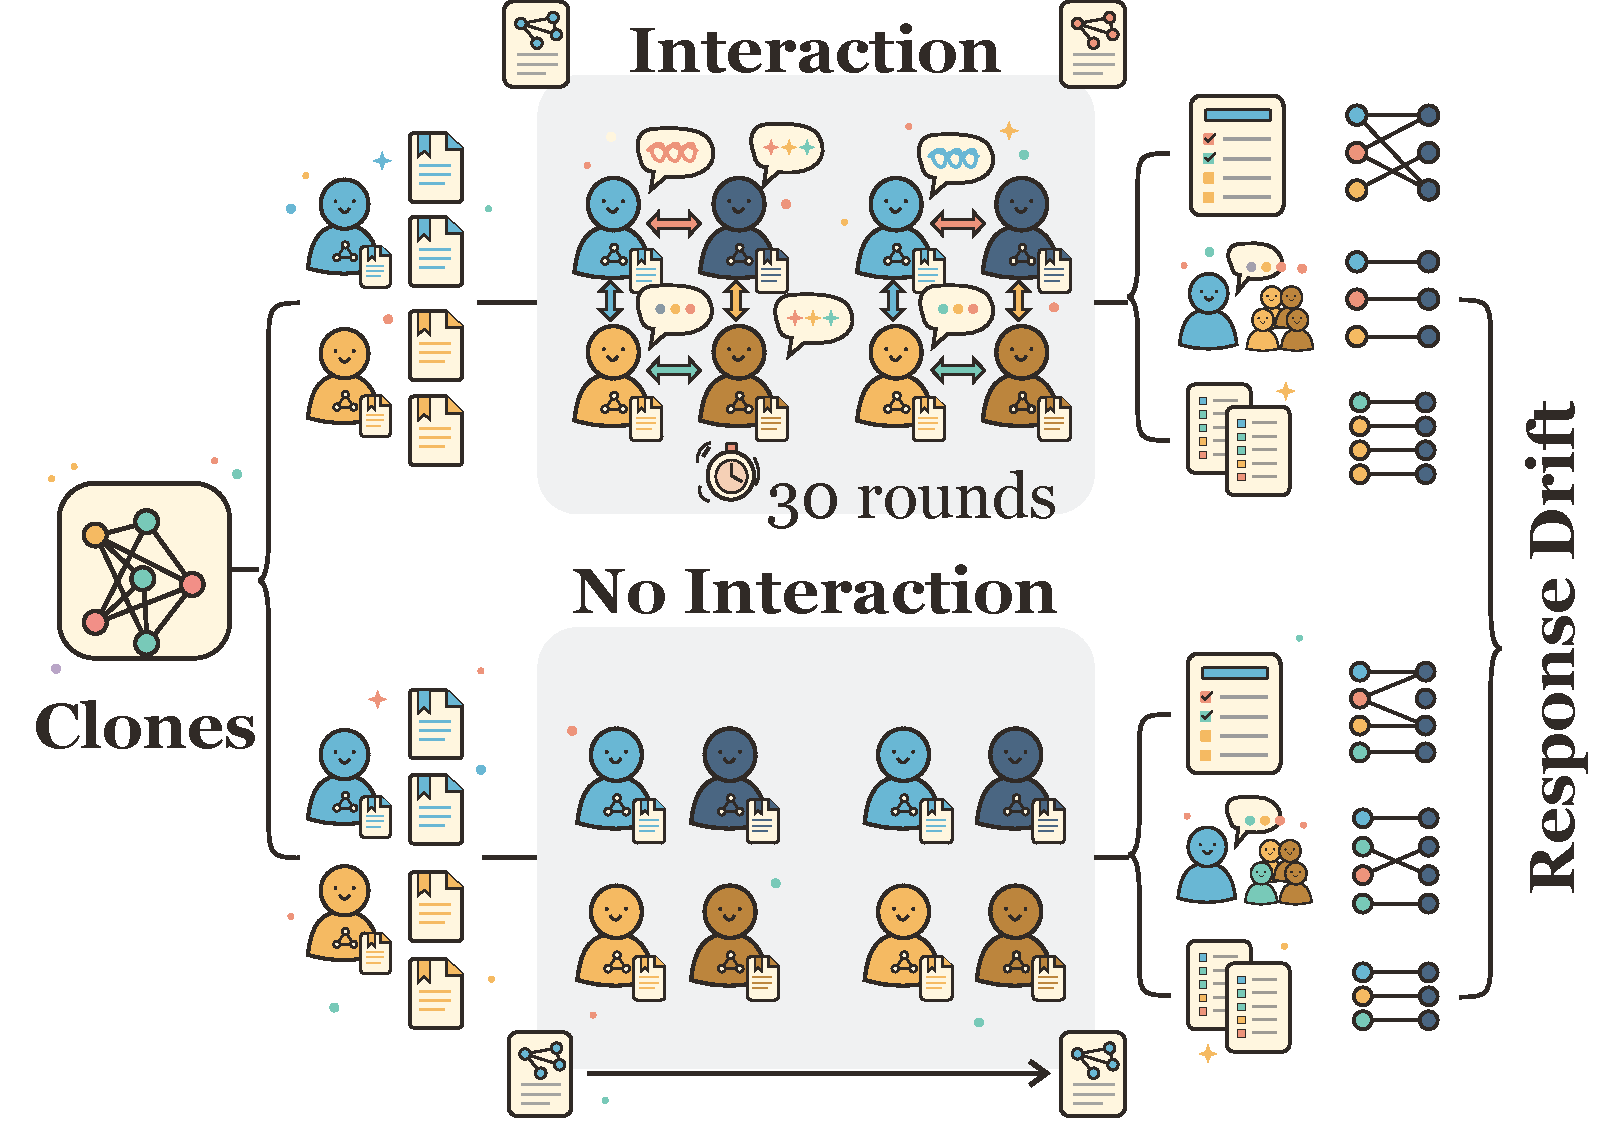
\includegraphics[width=\linewidth]{figures/fig1_teaser.pdf}
\caption{Interaction moves off-topic profiles.}\label{F0}
\vspace{-10pt}
\end{wrapfigure}

Many LLM systems build a population from copies of one model, including multi-agent debate~\citep{Du2024_MultiagentDebate,Liang2024_DivergentDebate,Du2024_Debate,Smit2024_MAD}, collaboration and evaluation frameworks~\citep{Li2023_CAMEL,Wu2024_AutoGen,Hong2024_MetaGPT,Chan2024_ChatEval}, simulated survey samples~\citep{Argyle2023,Aher2023_SimulateHumans}, and simulations of conflict, opinion, cooperation, and whole societies~\citep{Hua2024_WarAgent,OASIS,AgentSociety,Generative_Agents,Park2024_1000,Concordia,Li2024_SocioVerse,Chuang2024_OpinionDynamics,CisnerosVelarde2025_Funding,Piatti2024_GovSim,FlintAshery2025_Conventions,Anthis2025_SocialSim}. These studies treat the copies as comparable replicates of one system, even after many rounds of talk. If interaction changes the agents, each interacting population is one sample, and counting agents or posts as independent observations overstates the evidence~\citep{Hurlbert1984,Miller2024_ErrorBars}.

\begin{figure}[t]
\centering
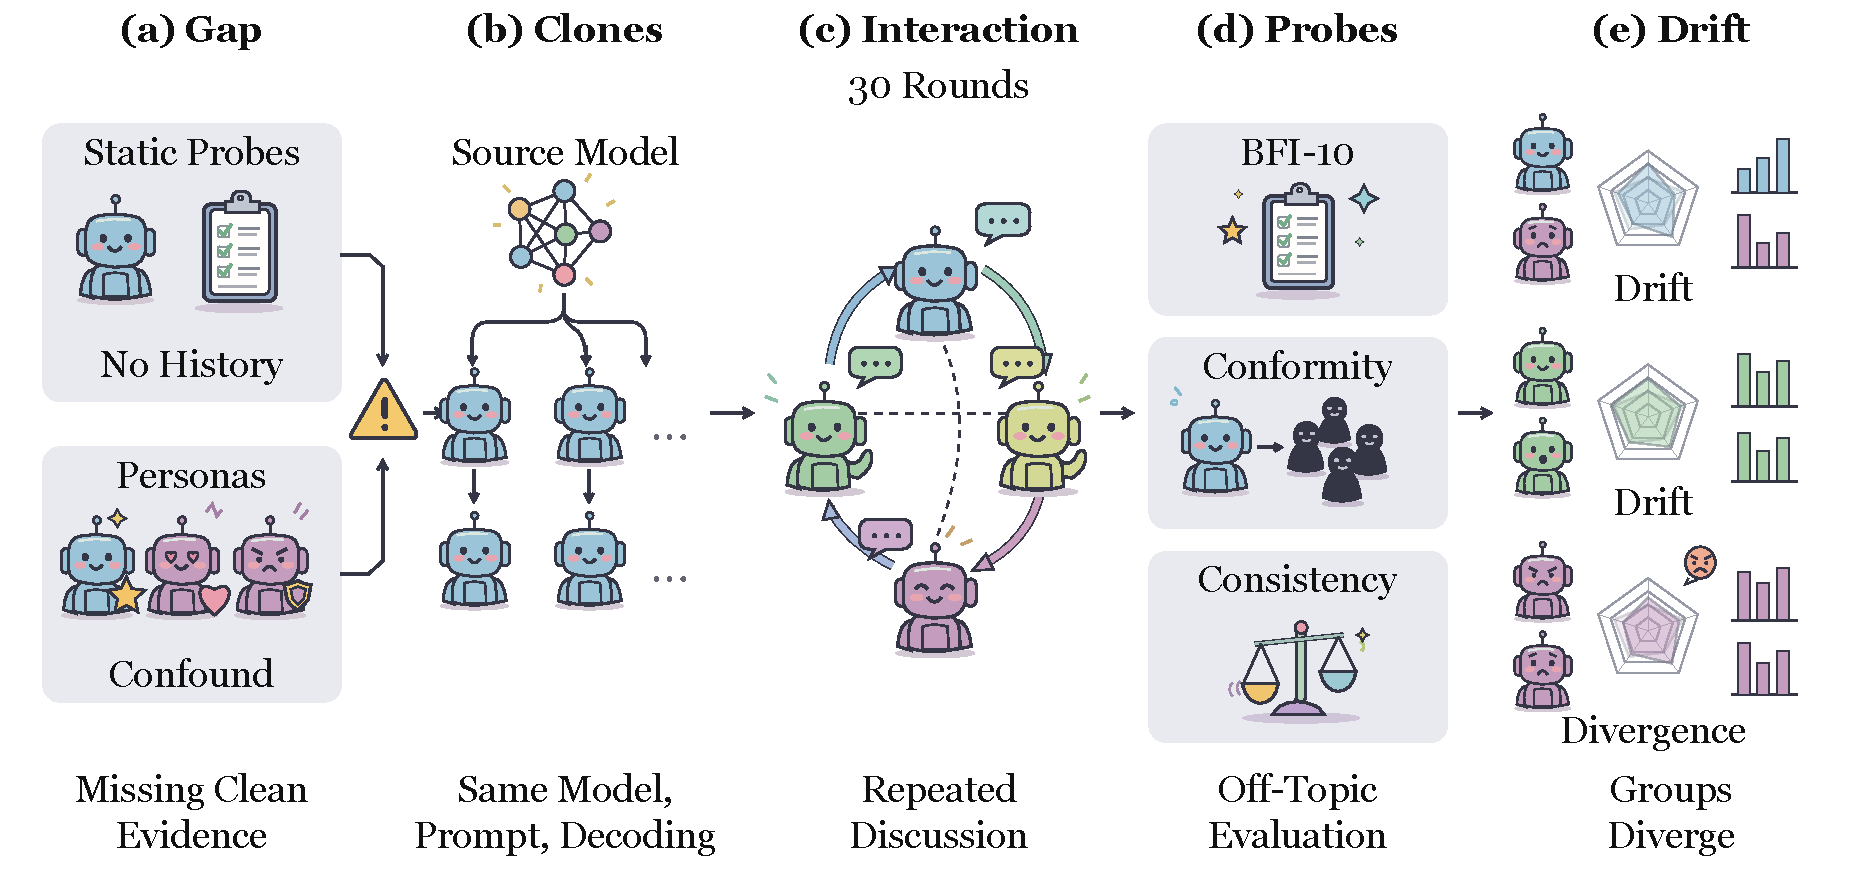
\includegraphics[width=\textwidth]{figures/fig2_overview.pdf}
\caption{The evaluation gap (a) and how SocCogEval tests transfer to unrelated probes (b--e).}\label{F1}
\end{figure}


This assumption still lacks a controlled test (Figure~\ref{F1}). Benchmarks score a frozen model on curated items or a short episode~\citep{MT-bench,AgentBench,ToMBench,Kim2023_FANTOM,Xu2024_OpenToM,CogBench,CogMir,PsychoBench}. Social simulations run long interactions but assign personas or opinions at the start, which mixes injected priors with the effect of interaction. Studies of drift, stability, and conformity measure the discussed task or the dialog itself~\citep{Li2024_PersonaDrift,Laban2025_LostMultiTurn,Kovac2024_StickToRole,Weng2025_Conformity,Potter2026,Rath2026_AgentDrift}, and personalities can emerge when undifferentiated agents communicate~\citep{Takata2024}. A controlled test has to meet three challenges. It must inject no differences at initialization, separate the effect of a brief from the effect of interaction, and use a probe unrelated to the discussed topic, analyzed at the level of the run.

SocCogEval meets them with controlled clones that share base model, system prompt, and decoding parameters, each holding at most one private brief. The Factorial Social Interaction Protocol (FSIP) crosses brief presence with 30 rounds of interaction, so the pure-interaction contrast $(C_2){-}(C_4)$ holds the brief fixed and toggles interaction (Figure~\ref{F0}). A solo-generation condition $C_6$ matches the call budget without any partner. The measurements follow three nested questions: do clones diverge on the discussed decision, do they predict exposed in-group peers better, and does the divergence transfer to an off-topic BFI-10 response profile?

\begin{figure}[t]
\centering
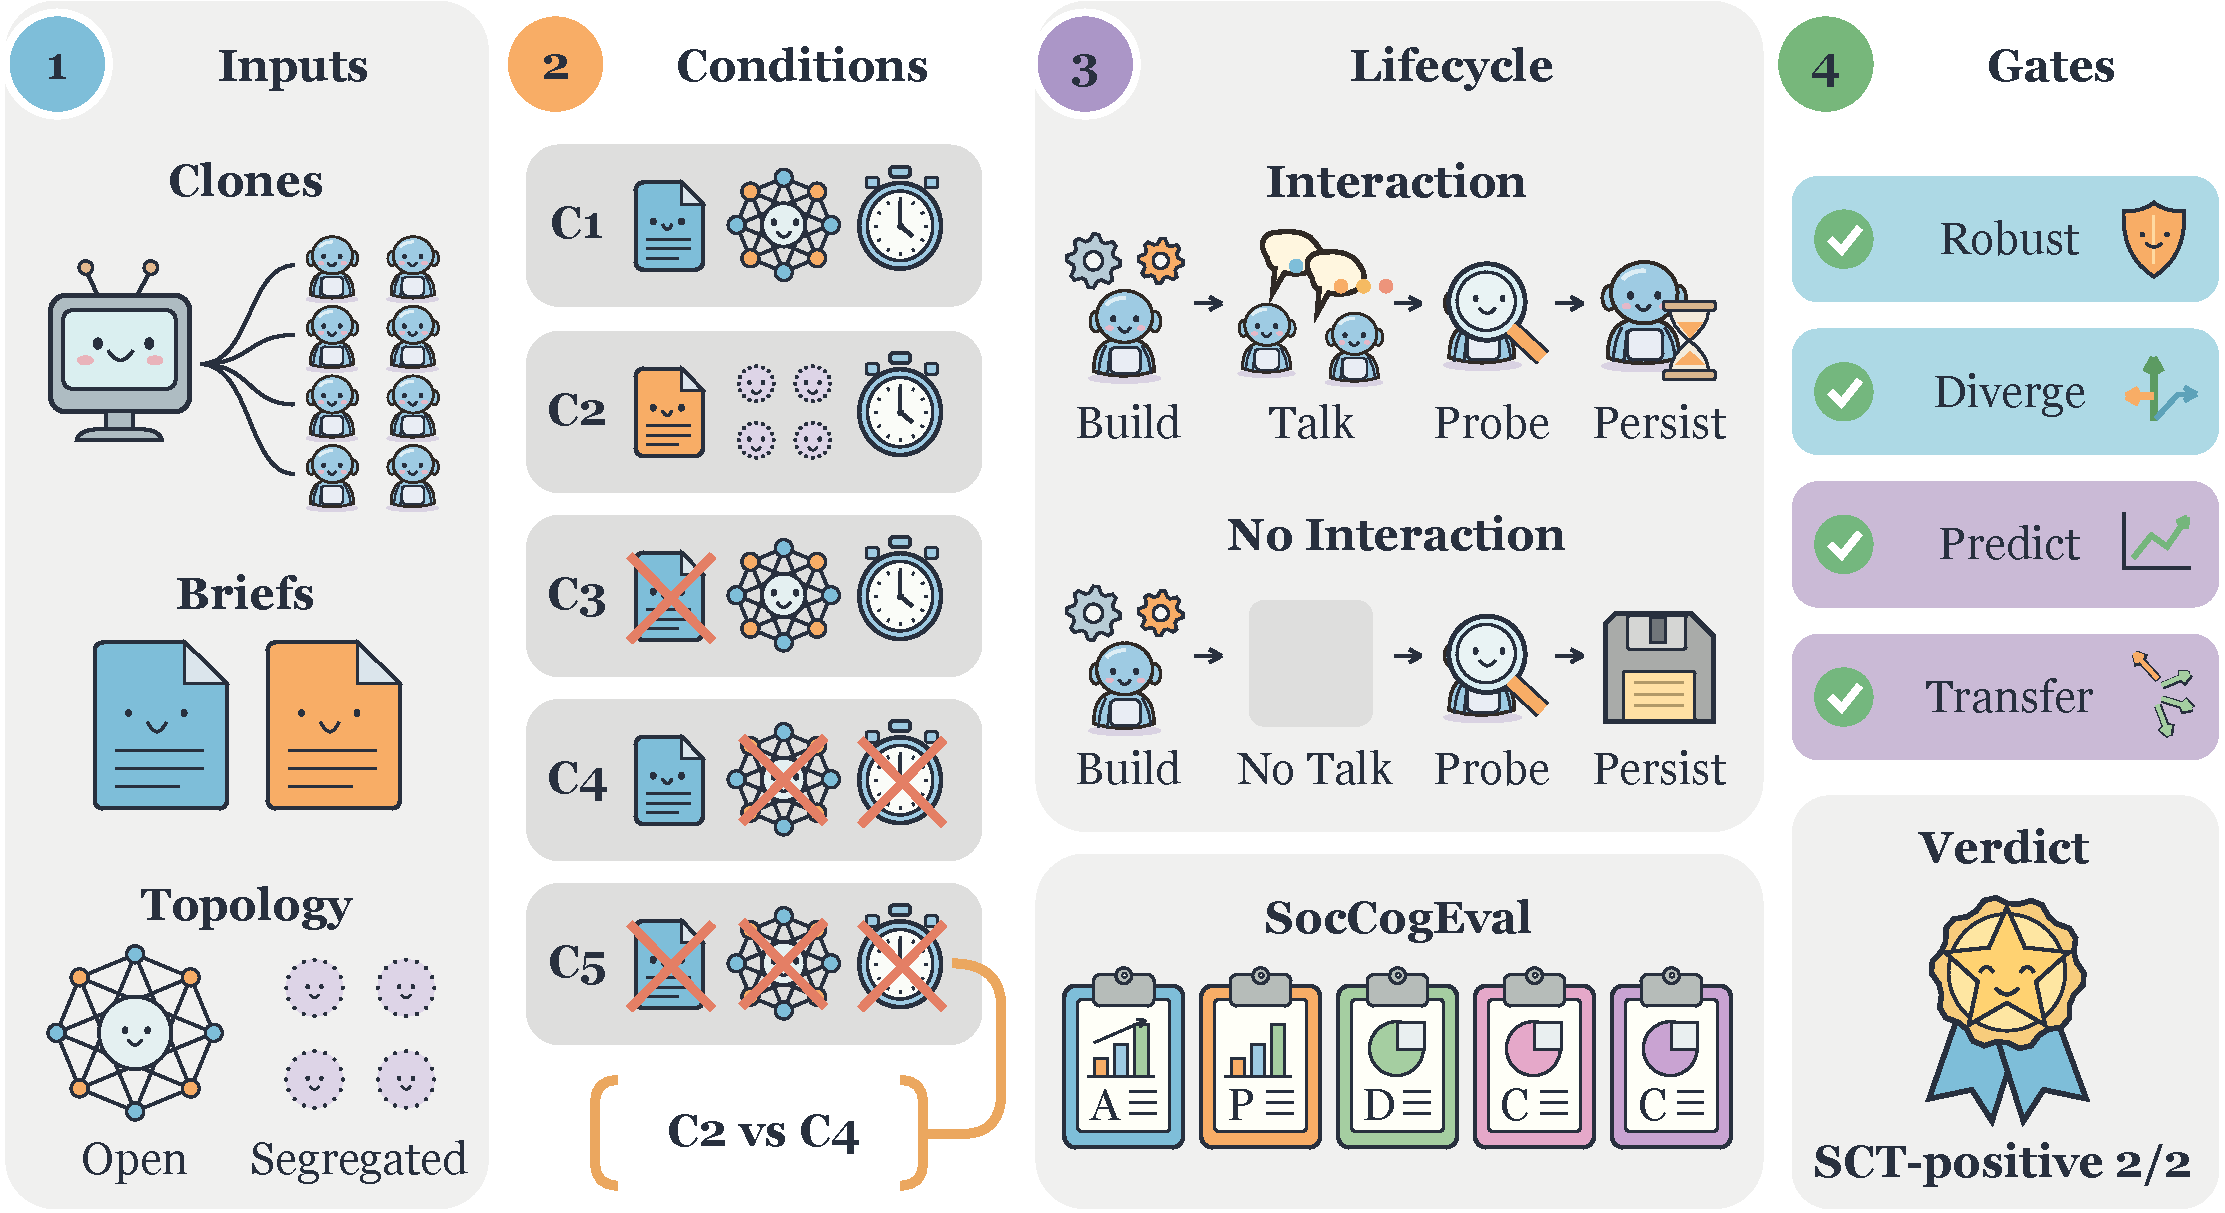
\includegraphics[width=\textwidth]{figures/fig3_fsip.pdf}
\caption{FSIP design and SocCogEval pipeline: $(C_2){-}(C_4)$ fixes the brief and toggles interaction.}\label{F2}
\end{figure}


Social interaction breaks replicate independence on the primary transfer outcome. On Qwen3-122B-FP8, the pure-interaction contrast is $\bar{\Delta}{=}{+}0.917$ BFI-10 L1 units on Greenfield and ${+}0.912$ on Riverton (run-level $p{=}0.0008$ and $0.0039$, $g{\approx}1.0$), about 0.18 Likert points per factor. Brief alone does not explain it, and it survives deterministic re-probing and a verbatim-history ablation without typed memory extraction. Solo generation reproduces part of the shift, while social interaction remains highest in both scenarios. Five more model variants give positive but uneven breadth, and all five have positive scenario-averaged $(C_2){-}(C_4)$ contrasts.

Our contributions are fourfold. (i) We define the Social Cognitive Transfer (SCT) task with three nested sub-tasks, Decision, Prediction, and Transfer. (ii) We propose FSIP, a five-condition design that isolates initialization noise, brief alone, interaction given brief, and brief given interaction, with a matched solo-generation condition $C_6$ as the mechanism boundary. (iii) We introduce SocCogEval, which combines task probes, a primary BFI-10 transfer instrument~\citep{Rammstedt2007_BFI10,PsychoBench}, secondary conformity and consistency probes~\citep{Asch1956_Conformity,CogMir}, and a contrast schema that turns measurements into causal claims. (iv) We show that social interaction breaks replicate independence on the primary transfer outcome, with cross-scenario stability and positive cross-model direction. The reported drift is restricted to Part 2 instruments unrelated to the discussion and gated by a three-part criterion (Section~\ref{sec:metrics}). SocCogEval is an identification protocol for this drift, not a benchmark of social-cognition capacity, and the drift is post-interaction response-profile drift, not personality change (Section~\ref{sec:exp-limits}).
